\chapter{Aromaticity as a Guide to Planarity in Conjugated Molecules and Polymers}

%%%%%%%%%%%%%%%%%%%%%%
\section{Introduction}

Organic semiconductors offer unique blends of physical and electronic properties along with the processability and fabrication potential of polymers and small molecules.\cite{Kuei2017, Swager2017} This combination opens up countless opportunities for new functional materials that can be tailored for specific applications.\cite{Mei2013, Muench2016, Someya2016, VanDeBurgt2018} One successful strategy for tuning molecular properties is adding pendent groups to the conjugated backbone; these ``noncovalent locks'' control molecular structure by inducing nonbonded interactions.\cite{Jackson2013, Cheng2016, Conboy2016, Huang2017} 
The goal is to create structures that prefer coplanar torsional configurations that maximize electron delocalization across the molecule or polymer (i.e. conjugation), and as a result improve electronic properties such as carrier mobility. 

While noncovalent locks have proven to be effective at creating planar structures, the exact nature of the interactions leading to planarity remain difficult to disentangle. A few reports have attempted to isolate and identify the fundamental interactions behind  noncovalent locking systems. For instance, Jackson et al. demonstrated that nontraditional hydrogen bonding (i.e. hydrogen bonding that involves less electronegative atoms such as C, S, and Cl) can play a predominant role in stabilizing planar configurations.\cite{Jackson2013} Nevertheless, many locking molecules such as 3,4-ethylenedioxythiophene (EDOT) and fluorinated thiophenes---which are utilized in state-of-the-art conjugated molecules and polymers\cite{Yum2014, Granstrom1995, Wijsboom2011, Gao2015, Gao2018, Jo2014, Li2015}---do not involve nontraditional hydrogen bonding. Conboy et al. confirmed the importance of heteroatom interactions in poly-EDOT (PEDOT) and similar molecules, but stated that a precise description of torsional energetics was unclear and speculated that electrostatics were responsible for the observed planarity.\cite{Conboy2016} 

%It is difficult to disentangle which interactions are responsible for configurational preferences, however, 
Aromaticity is a common chemical descriptor that can be used to simplify some of the underlying physics and provide novel insights into torsional energetics. A key objective of this communication is to highlight how the competition between aromaticity and conjugation\cite{Hernandez1994, Kertesz2005, Huang2017} influences planarity in organic electronic materials. We show that the introduction of popular noncovalent locks modifies aromaticity and drives structures towards planarity. Finally, we identity the specific hyperconjugation interaction that alters aromaticity and determines planarity.

%%%%%%%%%%%%%%%%%%%%%%%%%%%%%%%%
\section{Results and Discussion}

An illustrative example of the balance between ring aromaticity and conjugation is the torsion potential of bithiophene (BT) (Fig. 1). Dimers provide a computationally efficient and accurate representation of the torsion potential and trends in aromaticity observed in larger conjugated polymers (See SI)\cite{Dubay2012} and hence are used throughout this work. The aromaticity of individual rings is quantified using the multicenter bonding index (MCI),\cite{Giambiagi1990, Giambiagi2000} and the nucleus-independent chemical shift (NICS)\cite{Fallah-Bagher-Shaidaei2006, Chen2005} (see SI). We represent conjugation semi-quantitatively as the normalized relative bond length of the bridge C-C bond between rings; the rational being configurations with shorter bridge bonds are more conjugated.\cite{Daudey1980, Fernandez2006} Figure 1 (left side) clearly shows that the stabilizing effects of aromaticity and conjugation are in direct competition with one another. This agrees with a simple description based on atomic orbitals, where planar structures (0\textdegree \ cis and 180\textdegree \ trans) exhibit the most $p_z$-orbital overlap ($\pi$-bonding) and afford the most electron delocalization across the molecule. Whereas the torsioned structure at 90\textdegree \ will exhibit the least electron sharing between rings, and it possesses the highest ring aromaticity or electron delocalization within a ring. The non-planar global minimum (150\textdegree) in the torsion potential appears to be the balance between these two driving forces.

\begin{figure*}[hbt!]
    \centering
    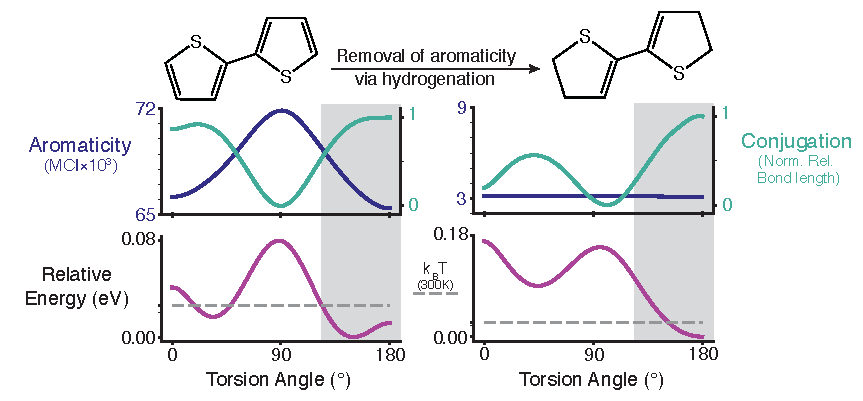
\includegraphics{figures/chap3/fig1_d2.pdf}
    \caption{Ring aromaticity, molecular conjugation, and relative energies are plotted as a function of torsion angle for bithiophene (BT) and hydrogenated bithiophene (hBT). Both BT and hBT structures are represented in the 180\textdegree \ (trans) configuration. Aromaticity and conjugation are directly opposed in BT and the balance between the two driving forces results in a non-planar torsional minimum around 150\textdegree. Hydrogenation of the terminal C-C double bonds essentially reduces aromaticity to zero, while preserving conjugation across the two rings. With aromaticity removed in hBT, torsional energetics mirror conjugation and there is a planar minimum at 180\textdegree. Aromaticity is defined as the multicenter bonding index (MCI$\times 10^3$) for one C-C-S-C-C thiophene ring. Only one ring is displayed because both BT and hBT are symmetric molecules. Conjugation is quantified as the normalized relative bridge C-C bond length. A value of 1 represents the shortest bond length and the highest conjugation, whereas 0 represents the longest bond and lowest amount of conjugation.}
    \label{fig:a_vs_c}
\end{figure*}

To test this hypothesis we removed aromaticity by hydrogenating the terminal C=C double bonds, leaving intact the conjugation across the rings (right side of Fig. 1). Once aromaticity was removed the torsional energetics essentially mirrored conjugation, and most importantly the global minimum in the torsion potential shifted to the planar 180\textdegree \ configuration. It is noteworthy that the inter-ring H$\cdots$S distance is reduced in hydrogenated bithiophene (hBT) (2.78\si{\angstrom} \ in the 180\textdegree \ configuration) compared to BT (2.93\si{\angstrom} \ in the 180\textdegree \ configuration), which reduces concern that the 150\textdegree \ torsional minimum in BT is due to steric repulsion between H$\cdots$S. This conclusion is supported with through-space calculations and noncovalent interaction (NCI) analysis\cite{Johnson2010, Contreras-Garcia2011} in the SI. Establishing aromaticity as a driving force in torsional energetics is fundamental for understanding structure; additionally, if aromaticity can be modified or controlled it may represent a design opportunity.

Having demonstrated the important role of aromaticity in directing torsion angles, we were motivated to explore the role of aromaticity in known planar systems with noncovalent locks. We discovered a number of reported noncovalent locks modify aromaticity. As observed in the top of Fig. 2 both  3,3'-difluorobithiophene (F2-BT) and bis-EDOT (BEDOT) exhibit a coplanar torsional minimum at 180\textdegree \ accompanied by an increase in aromaticity near 180\textdegree. As expected, conjugation is minimized at 90\textdegree \ and a maximized at 180\textdegree, it has been left out of Fig. 2 for clarity. For torsional energetics the magnitude of aromaticity is less important than the change in aromaticity. For example, if aromaticity is constant across all torsion angles there is no torsional driving force. As a result, we are interested in the change in aromaticity between 90-180\textdegree. 

To further investigate the modification of aromaticity we systematically added fluorine at different ring positions (bottom of Fig. 2). Notably, aromaticity increases near 180\textdegree \ in ring 2 (the ring without F added) of 3F-BT similarly to that of BEDOT and F2-BT in the top of Fig. 2. With only one added fluorine the aromaticity of both ring 1 and ring 2 need to be characterized because the molecule is no longer symmetric. When fluorine is added to ring 1---regardless of the position---it reduces the magnitude of aromaticity but preserves the shape of the curve (bottom left of Fig. 2), essentially reducing the underlying function by a constant. This is consistent with earlier reports that adding electron withdrawing substituents to an aromatic ring reduces the overall aromaticity.\cite{Krygowski2014} Naively, one might expect all thiophene rings without F added to be similar, and this is largely true for ring 2 of BT and 4F-BT but as mentioned ring 2 aromaticity is modified in 3F-BT. This result indicates that there is a noncovalent inter-ring interaction between F$\cdots$S causing the change in aromaticity.

Using Natural Bonding Orbital (NBO) analysis we identify the key interaction responsible for the modification of aromaticity and for stabilizing the planar 180\textdegree \ configuration (Fig. 3). Our through-space calculations for F$\cdots$S and O$\cdots$S indicate that both would be repulsive at the respective relaxed separation distance present in the 180\textdegree \ configuration of F2-BT and BEDOT (see SI). Thus, it is clear that some other interaction involving X$\cdots$S is stabilizing the steric effects in order for the 180\textdegree \ configuration to be energetically favorable. NBO perturbation analyses revealed a 3-center-2-electron interaction between a heteroatom lone pair and a C-S antibonding orbital ($\sigma^{*}_{C-S}$) pictured in the top of Fig. 3. Details on specific energies are provided in the SI. Similar interactions have been reported for the association of supramolecules.\cite{Cozzolino2005} Conboy et al. mentioned this type of interaction as a possible source of attraction in BEDOT-like molecules, but dismissed it due to a lack of bond length correlations across a series of related molecules.\cite{Conboy2016}

In order to confirm the importance of the 3-center-2-electron interaction we utilized the NBO deletion method\cite{NBO6}, which has been used previously to deconvolute torsional energetics.\cite{Pophristic2001} Because the NBO deletion method necessitates the use of restricted Hartree-Fock (RHF) we recalculated the torsion potentials with RHF to ensure qualitatively similar behavior to the higher level of theory ($\omega$B97x-D). Then using the RHF deletion method, we removed the C-S antibonding orbitals ($\sigma^{*}_{C-S}$) on both rings, which eliminates hyperconjugation. Remarkably, removing hyperconjugation altered the torsional energetics in both BEDOT and F2-BT such that the planar 180\textdegree \ configurations are no longer favorable (as shown in Figure 3), most likely due to the steric repulsion that exists. We characterize these as hyperconjugation interactions because they result in electron delocalization across the molecule and there is a history of hyperconjugation impacting torsional energetics.\cite{Pophristic2001, R.Rablen1999} This result provides strong evidence that hyperconjugation is the critical interaction responsible for the locking behavior in these molecules and polymers.

%%%%%%%%%%%%%%%%%%%%
\section{Conclusion}

Using a variety of computational techniques we have demonstrated that aromaticity is a useful descriptor to help understand the complex interactions which lead to the structure of conjugated molecules and polymers. In general, aromaticity is stabilizing and energetically favorable, and in extended conjugated molecules and polymers ring aromaticity prefers torsioned or non-planar configurations because it confines delocalized electrons within a ring instead of delocalizing them across the entire molecule or polymer. As such, aromaticity directly competes with conjugation, also known to be stabilizing and energetically favorable. BT is an ideal system to exemplify this competition, and ultimately we identify a balance between the two factors that results in a non-planar minimum energy configuration. Planarity and conjugation are vital for the electronic properties of conjugated materials so minimizing the driving force from aromaticity is industrially relevant. We find that aromaticity can indeed be beneficially modified through pendent group additions or noncovalent locks such as F2-BT and BEDOT. In both examples, a heteroatom interacts with an adjacent ring and increases its aromaticity at torsional angles near 180\textdegree \ where the atoms are the closest together. To probe the exact nature of this interaction we identified and removed hyperconjugation between a heteroatom (i.e. F and O) lone pair and the C-S antibonding orbital on the adjacent ring, concluding that hyperconjugation is responsible for the changes in aromaticity and for the resulting planarity or locking behavior. We anticipate that the structural insights and methods presented here are applicable to a wide range of conjugated molecules and polymers, and will open the door to new and unforeseen advances in our ability to design functional organic electronic materials.

%%%%%%%%%%%%%%%%%%%%%%%%%%%%%%%
\section{Computational Methods}

All quantum chemistry calculations were performed with Gaussian 16 unless otherwise noted.\cite{g16} The default level of theory was $\omega$B97x-D with the def2-TZVPP basis set.\cite{Chai2008, Weigend2005} The general procedure for calculating torsion potentials started with an unconstrained geometry relaxation followed by a frequency calculation to ensure no substantial imaginary frequencies existed. Then the relaxed geometry was rotated around the central C-C bond, fixing the C-C-C-C torsion every 10\textdegree \ for a constrained geometry optimization. An additional torsional constraint was used for hydrogenated calculations (See SI). MCI aromaticities were computed with the natural atomic orbital basis from NBO6 for all 5 member (C-C-S-C-C) rings at each torsional geometry using Multiwfn.\cite{Lu2012} NBO analysis was performed using NBO6.\cite{NBO6} All RHF and RHF NBO orbital deletions were done with Gaussian 09\cite{g09} and NBO6 again using the def2-TZVPP basis set. RHF NBO orbital deletions were single point calculations utilizing relaxed RHF geometries. Isosurface images were made with VMD,\cite{HUMP96} and all plotting utilized Matplotlib and cubic spline interpolation via SciPy.\cite{Jones} 